\documentclass{article}
\usepackage[utf8]{inputenc}
\usepackage{amsmath}
\usepackage{amssymb}
\usepackage{color}
\usepackage{amsmath}
\newtheorem{theorem}{Theorem}[section]
\newtheorem{definition}{Definition}[section]
\newcommand{\R}{\mathbb{R}}
\newcommand{\norm}[1]{\left\lVert#1\right\rVert}


\newcommand{\myint}{\int\limits}
\newcommand{\diff}[1]{\, d#1}
\newcommand{\vect}[1]{\mathbf{#1}}
\usepackage{mleftright}
\newcommand{\of}[1]{\mleft( #1 \mright)}
\newcommand{\ddt}[1]{\partial_t #1}
\newcommand{\vth}{v_\textrm{th}}
\newcommand{\reals}{\mathbb{R}}
\newcommand{\RR}{\mathbb{R}}
\newcommand{\vr}{v}
%\newcommand{\vtheta}{\theta_{\vect{v}}}
%\newcommand{\vphi}{\varphi_{\vect{v}}}
%\newcommand{\vr}{v_{r}}
\newcommand{\vtheta}{v_{\theta}}
\newcommand{\vphi}{v_{\varphi}}
\newcommand{\vomega}{v_{\omega}}
\newcommand{\vrunit}{\hat{\vect{v}}_{r}}
\newcommand{\vthetaunit}{\hat{\vect{v}}_{\theta}}
\newcommand{\vphiunit}{\hat{\vect{v}}_{\varphi}}
\newcommand{\lp}[2]{L^{(#1)}_{#2}}
\newcommand{\lph}[2]{\tilde{L}^{(#1)}_{#2}}
\newcommand{\bfun}[2]{\Phi^{(#1)}_{#2}}
\newcommand{\tfun}[2]{\Psi^{(#1)}_{#2}}
\newcommand{\nfun}[2]{N^{(#1)}_{#2}}
\newcommand{\maxp}[2]{P^{(#1)}_{#2}}
\newcommand{\diffm}[3]{D^{(#1)}_{#2,#3}}
\newcommand{\myint}[2]{\int\limits_{#1}^{#2}}
\newcommand{\diff}[1]{\, d#1}
\newcommand{\vect}[1]{\mathbf{#1}}
\usepackage{mleftright}
\newcommand{\of}[1]{\mleft( #1 \mright)}
\newcommand{\ddt}[1]{\partial_t #1}
\newcommand{\vth}{v_\textrm{th}}
\newcommand{\reals}{\mathbb{R}}
\newcommand{\RR}{\mathbb{R}}
\usepackage{pgfplots}
\pgfplotsset{compat=newest}
\usepackage{float}
\usepackage{algorithm}
\usepackage{algpseudocode}

\title{Scalable deterministic numerical methods for the Boltzmann equation}
%\author{Milinda Fernando}
%\date{February 2014}

\begin{document}

%\begin{titlepage}
\maketitle
%\end{titlepage}

\section{Boltzmann Equation summary}
The Boltzmann equation is a nonlinear integro-differential equation that describes the evolution of the particle density function $f : \R^3 \times \R^3 \times \R \rightarrow \R^{+}_0$. Independent variables for the above density function denotes, time ($t$), position vector ($x$), and the velocity ($v$). For a fixed time $t$, $f(x,v,t)dx dv$ represent the number of particles for the phase space volume element $dxdv$. 

We can write the Boltzmann equation in the absence of external force field can be written as below. 
\begin{equation}
    \partial_t f + v\cdot \nabla_x f = \frac{1}{\epsilon}Q(f,f) \text{ for } x,v \in \R^3 \label{eq:be}
\end{equation}
In the presence of external force field (e.g., electromagnetic field) $L(x,t) : \R^3 \times \R \rightarrow \R$, the full Boltzmann equations can be written as, 
\begin{equation}
    \partial_t f + v\cdot \nabla_x f  + L \cdot \nabla_v f = \frac{1}{\epsilon}Q(f,f) \text{ for } x,v \in \R^3 \label{eq:be_full}
\end{equation}

The $\epsilon$ is known as the Knudsen number (dimensionless number, $\epsilon > 0$), $Q$ is the collision operator. 

\textbf{Note}: Unless stated otherwise, $v^\prime,v_*^\prime$ denotes the post-collision velocities and $v,v_*$ denotes the pre-collision velocities of a binary collision.

The collision operator (i.e., capture the physics of the collisions) can be broken up to two main parts, 
\begin{enumerate}
    \item Gain term ($C^+(f,f)$) : For a fixed $(t,x)$ how many particles created with velocity $v$.
    \item Loss term ($C^-(f,f)$) : For a fixed $(t,x)$ how many particles are lost with velocity $v$.
\end{enumerate} which are defined as follows. 

\subsection{Multi-species binary collisions}
\label{sec:multispecies_collissions}
Let $f_e,f_o$, denotes the distribution functions for electrons and heavy particles respectively. 



% \begin{align}
%     C^{+}(f,f) &= \int_{\R^3}\int_{S^2} B(|v-v_*|,\omega) f(v^\prime)f(v_*^\prime) d\omega dv_* \\
%     C^{-}(f,f) &= \int_{\R^3}\int_{S^2} B(|v-v_*|,\omega) f(v)f(v_*) d\omega dv_* 
% \end{align}

% The collision operator then defined as, 
% \begin{equation}
%     \begin{split}
%         C(f,f) = C^{+}(f,f) - C^{-}(f,f) %= \\ \int_{\R^3}\int_{S^2} B(|v-v_*|,\theta)(f(v^\prime)f(v_*^\prime) - f(v)f(v_*) ) d\omega dv_*    
%     \end{split}
% \end{equation}

\section{Electron - Ar collisions}
\label{sec:col_op_torch}

Assuming, that the neutral Ar atoms have $n_0\delta(0)$ distribution in the velocity space, where $n_0$ denotes the Ar density, and collision kernel $B$ approximation from experimental data, the above collusion operator simplifies to,
\begin{equation}
    C(f) = n_0 \int_{S^2} (f(v^\prime) - f(v)) \norm{v} \sigma(\norm{v},\omega) d\omega
\end{equation}

\subsection{Total and differential cross section}
For a given total cross section value, the differential cross section, can be computed as follows\cite{vahedi1995monte}, where $\varepsilon= \frac{1}{2}mv^2$
\begin{equation}
    \sigma(\varepsilon,\chi) = \frac{\sigma(\varepsilon)\varepsilon}{4\pi (1 + \varepsilon \sin^2(\chi/2))\ln(1+\varepsilon)} 
\end{equation}

\subsection{Post-collision velocity}
The scattering velocity direction is computed based on using following notations. Assumes vector coordinates w.r.t. basis $\hat{e_i},\hat{e_j}$ and $\hat{e_k}$.

\begin{itemize}
    \item $v_0$, $\hat{v_0}$ : pre-collision velocity, unit vector along $v_0$
    \item $v_1$, $\hat{v_1}$ : scattered (post-collision) velocity, unit vector along $\boldmath{v_1}$
    \item $\chi$ : scattering angle, i.e., the angle between vectors, $\hat{v_1}$ and  $\hat{v_0}$
    \item $\phi$ : angle between $v_1$ projection onto $v_0 \times(v_0 \times e_i)$, $v_0 \times e_i$ plane, and vector $v_0 \times(v_0 \times e_i)$
    \item $\theta$ : angle between $\hat{v_0}$ and $\hat{e_i}$, i.e., $cos\theta = \hat{v_0} \cdot \hat{e_i}$
\end{itemize}
The angle $\theta$ can be computed from $v_0$, and $\chi,\phi$ are taken to represent the solid angle for the collision event. The scattered velocity can be decomposed along the orthonormal basis vectors, $\hat{E_0}=\hat{v_{0}}$, $\hat{E_1}= \cfrac{\hat{v_0}\times e_i}{\sin\theta}$, and $\hat{E_2}= \hat{v_0}\times \hat{E_1}$. Therefore, the scattered direction unit vector can be written, 

\begin{equation}
    \hat{v_1} = \cos\chi \hat{v_0} + \sin\chi sin\phi (\frac{\hat{v_0}\times \hat{e_i}}{\sin\theta}) + \sin\chi cos\phi (\hat{v_0}\times \frac{\hat{v_0}\times \hat{e_i}}{\sin\theta}) \label{eq:scatter}
\end{equation}
We can see that, $\hat{v_1}\cdot \hat{v_1}=1$, and $\hat{v_1} \cdot \hat{v_0}= \cos\chi$.
When $\theta = 0 $, we can pick $\hat{E_0}=\hat{e_i}$, $\hat{E_1}=\hat{e_j}$ and $\hat{E_2}=\hat{e_k}$ as the basis to derive the scattering direction. 

In spherical coordinates, for a given incident vector $(v_r,\theta,\phi)$ that is not parallel to $\hat{e_i}$,  and scattering angle $(\chi,\gamma)$, we can compute the direction of the scattered particle as 

\begin{align}
    \theta^\prime &= \tiny \left\{\cos ^{-1}\left(\frac{\cos (\theta ) \left(\cos (\gamma ) \sin (\theta ) \sin (\chi ) \cos (\phi )+\cos (\chi ) \sqrt{1-\sin ^2(\theta ) \cos ^2(\phi )}\right)-\sin (\gamma ) \sin (\theta ) \sin (\chi ) \sin (\phi )}{\sqrt{1-\sin ^2(\theta ) \cos ^2(\phi )}}\right)\right\} \\
    \phi^\prime &= \tan ^{-1}\left(\frac{\sin (\chi ) \left(\cos (\gamma ) \sin ^2(\theta ) \sin (\phi ) \cos (\phi )+\sin (\gamma ) \cos (\theta )\right)+\sin (\theta ) \cos (\chi ) \sin (\phi ) \sqrt{1-\sin ^2(\theta ) \cos ^2(\phi )}}{\sin (\theta ) \cos (\chi ) \cos (\phi ) \sqrt{1-\sin ^2(\theta ) \cos ^2(\phi )}-\cos (\gamma ) \sin (\chi ) \left(\sin ^2(\theta ) \sin ^2(\phi )+\cos ^2(\theta )\right)}\right)
\end{align}

If the incident vector is parallel to the $\hat{e_i}$, we can compute the above, 
\begin{align}
    \theta^\prime &=\left\{\cos ^{-1}(\cos (\gamma ) \sin (\chi ))\right\} \\
    \phi^\prime &=\tan ^{-1}(\sin (\gamma ) \tan (\chi )) \\
\end{align}




\subsection{G0 : $e + Ar \rightarrow e + Ar$ collision operator}
\begin{equation}
    C_{G0}(f) = n_0 \int_{\chi} \int_{\phi} (f(v_1) - f(v_0)) \norm{v_0} \sigma_{G0}(\norm{v_0},\omega) \sin\chi d\phi d\chi
\end{equation}

Let $\varepsilon_0 = 1/2 m \norm{v_0}^2_2$ , $\varepsilon_1 = 1/2 m \norm{v_1}^2_2$, for inelastic collisions the energy lost, modeled based on \cite{vahedi1995monte}, (relative energy loss)
\begin{equation}
    \Delta \varepsilon = \frac{2m(1-cos\chi)}{M}
\end{equation} where, $m,M$ denotes the mass of the electron and the argon atom. Therefore the magnitude of the scattered velocity, can be written as, 
\begin{equation}
    \norm{v_1} = \norm{v_0} \sqrt{1- \frac{2m(1-cos\chi)}{M}}
\end{equation} where the direction of $v_1$ is specified by $\hat{v_1}$ in (\ref{eq:scatter}).

\subsection{G1 : $e + Ar \rightarrow e + Ar^*$ collision operator}
\begin{equation}
    C_{G1}(f) = n_0 \int_{\chi} \int_{\phi} (f(v_1) - f(v_0)) \norm{v_0} \sigma_{G1}(\norm{v_0},\omega) \sin\chi d\phi d\chi
\end{equation}
Let $\varepsilon_{exc}$ be the energy threshold to trigger an excitation reaction, then we can write, 
\begin{align}
    \frac{1}{2} m v_0 ^2  - \varepsilon_{exc} &= \frac{1}{2} m v_1 ^2 \\
    \norm{v_1} &= \sqrt{\norm{v_0}^2 - \frac{2\varepsilon_{exc}}{m}}
\end{align} where the direction of $v_1$ is specified by $\hat{v_1}$ in (\ref{eq:scatter}). Note that, we use excitation threshold of $\varepsilon_{exc}=11.5eV$.

\subsection{G2 : $e + Ar \rightarrow e + Ar^+ + e$ collision operator}
\begin{itemize}
    \item $v_1$ : velocity of the scattered electron
    \item $v_2$ : velocity of the ejected electron from Ar. 
\end{itemize}
\begin{equation}
    C_{G2}(f) = n_0 \int_{\chi} \int_{\phi} (f(v_1) + f(v_2) - f(v_0)) \norm{v_0} \sigma_{G2}(\norm{v_0},\omega) \sin\chi d\phi d\chi
\end{equation}

Let $\varepsilon_{ion}$ be the energy threshold for the ionization reaction, then as in \cite{vahedi1995monte} we split the $\varepsilon_0-\varepsilon_{ion}$ equally among scattered and the ejected electron. i.e., $\varepsilon_1 = 0.5 (\varepsilon_0-\varepsilon_{ion})$, $\varepsilon_2 = 0.5 (\varepsilon_0-\varepsilon_{ion})$. Therefore, we can derive the velocity magnitudes of the scattered and ejected electrons as follows. 
\begin{align}
    \norm{v_1} &= \sqrt{\frac{1}{2}\norm{v_0}^2 - \frac{\varepsilon_{ion}}{m}}\\
    \norm{v_2} &= \sqrt{\frac{1}{2}\norm{v_0}^2 - \frac{\varepsilon_{ion}}{m}}
\end{align}
The direction of $v_1$ is given by $\hat{v_1}$ as in (\ref{eq:scatter}) and the direction of the $v_2$ derived based on the momentum conservation, assuming the momentum change in the Ar atom is negligible. 
\begin{align}
    m v_0 + M v &= Mv + m v_1 + m v_2  \\
    \hat{v_2} &= \frac{v_0 - v_1}{\norm{v_0 - v_1}}
\end{align}



\section{Maxwell-Boltzmann distribution (Maxwellian)}
\label{sec:maxwellian}
A particularly important velocity distribution function is the Maxwell-Boltzmann distribution, or Maxwellian. It describes the spread of velocities for a gas which is in thermal equilibrium. Maxwellian in $d$ dimensional velocity space can be written as,

\begin{equation}
    M(v) = A \exp(-\frac{mv^2}{2k_BT})
\end{equation}
using the number density equation, we can derive the coefficient $A$ as follows, 
\begin{equation}
M(v) = \frac{n}{(\sqrt{\pi}v_{th})^d} \exp{(-(\frac{v}{v_{th}})^2)}    
\end{equation} where, $v_{th}$ defined as, 
\begin{equation}
    v_{th} = \sqrt{\frac{2kT}{m}}
\end{equation}



%\section{Splitting the Boltzmann}
%\label{sec:split}

\section{Collision Operator}
\label{sec:collision_operator}
The term $v\cdot \nabla_x f$ makes the distribution $f(v)$ at fixed $(t,x)$ coupled with $f(v)$ defined in neighboring $x$. In operator splitting methods, Boltzmann equation is split in to ``transport'' and ``collision'' part. First we are going to focus on the collision part, given by, 
\begin{equation}
    \partial_t f = \frac{1}{\epsilon}C(f,f) \label{eq:col_op}
\end{equation}
% Note that without the transport term, for fixed $(t,v)$, for $x\neq x_*$ $f(x)$ and $f(x_*)$ can be evolved independently decoupled way. \emph{This allows, spatially subdivision based parallelization algorithms for the Boltzmann equation.}

% \subsection{Properties of the collision operator}
% \label{subsec:collision_op_properties}
% For a given $\R^d$ velocity space,
% \begin{theorem}
%     The Boltzmann collision operator conserves few of it moments, namely, mass, momentum, and energy.
%     \begin{align}
%         \int_{\R^d} Q(f,f) dv  = 0 \\
%         \int_{\R^d} Q(f,f) v dv  = 0 \\
%         \int_{\R^d} Q(f,f) |v|^2dv  = 0 \\
%     \end{align}
% \end{theorem}

% The solution for (\ref{eq:col_op}) evolves towards steady state, defined as the Maxwellian, which is given by, 
% \begin{equation}
%     f_{\infty}(v) = \frac{\rho}{(2\pi T)^{d/2}} \exp{-\frac{|V-v|^2}{2T}}
% \end{equation} where, the Maxwellian depends on the quantities computed from the initial distribution. 

% \begin{itemize}
%     \item \textbf{Density} : $\rho = \int_{\R^d} f(v) dv$ 
%     \item \textbf{Mean/Bulk velocity}: $V=\frac{1}{\rho} \int_{\R^d} v f(v) dv$ 
%     \item \textbf{Temperature}: $T= \frac{1}{3\rho} \int_{\R^d} |V-v|^2 f(v) dv$
% \end{itemize}

\section{0D space collision operator for electron-neutral collisions}
\label{sec:electron_neutral_pc}
Let $f_e(v,t)$ be the electron density and $f_o(v,t)=\delta(v)$ for all $(t,x)$. Then the evolution of the $f_e$ can be written as, 
\begin{equation}
    \partial_t f_e(v,t) = C(f_e,f_0)
\end{equation}
Let $(v^\prime,v_*^\prime) \rightarrow (v,v_*)$ be the pre and post collision velocities. The assumption $f_o(v,t)=\delta(v)$, implies neutral particles are mostly centered at velocity $0$. We can write the pre collision velocities as, $v^\prime=v^\prime(v,\omega)$. 

With these assumptions, the generic collision operator, for fixed time $t$ can be simplified for follows. 
\begin{align}
    C(f_e,f_0) &= \int_{\R^3}\int_{S^2} B(|v-v_*|,\omega)(f_e(v^\prime)f_0(v_*^\prime) - f_e(v)f_0(v_*) ) d\omega dv_*
\end{align}
Change of the integral order (assumes that the integral is finite) with properties of the Dirac's delta function, we can write, 
\begin{align}
    C(f_e,f_0) &= \int_{S^2} B(|v|,\omega)(f_e(v^\prime) - f_e(v)) d\omega
\end{align}

Then we can write the final evolution equation as, 
\begin{equation}
    \partial_t f_e(v,t) = \int_{S^2} B(|v|,\omega)(f_e(v^\prime,t) - f_e(v,t)) d\omega
\end{equation}

Since we know the above evolution will reach the Maxwellian at $t\rightarrow \infty$, we approximate $f_e(v,t)$ as follows, where $M(v)$ denotes the Maxwellian, 
\begin{equation}
    f_e(v,t) = M(v)[1 + h(v,t)] \label{eq:maxwelian}
\end{equation}
The idea is that when $t\rightarrow \infty$ the time dependent, $h(v,t)\rightarrow 0$.
Assuming that $\phi(v)$ is our test function with required properties. We can write the variational form for the above as, 
\begin{equation}
    \frac{\partial}{\partial t} \int_{\R^3} f_e(v,t) \phi(v) dv = \int_{\R^3} \int_{S^2} B(|v|,\omega)(f_e(v^\prime,t) - f_e(v,t)) \phi(v) d\omega dv \label{eq:0d_wf}
\end{equation}

Let $P_i(v)$ be orthonormal polynomial basis with the weighted inner product in the velocity space, where $w(v)$ denotes tha weight function. 
\begin{align}
    \int_{V} w(v)P_i(v)P_j(v) dv &= k_i\delta_{ij}
\end{align}

Assuming finite dimensional expansion for fixed time $t$, on $f(v,t)$, we can write, 
\begin{equation}
    f(v,t) \approxeq \bar{f}(v,t) = M(v)\sum_{j=0}^{N_v} f_j(t) P_j(v) \label{eq:basis_expansion}
\end{equation}

% Substituting (\ref{eq:basis_expansion}) to (\ref{eq:0d_wf}) we can write, 
% \begin{align}
%     \partial_t \int_{\R^3} w(v)h(v,t)\phi(v) dv &=  \int_{\R^3} \int_{S^2} (M(v^\prime) - M(v)) \phi(v) B(|v|,\omega) d\omega dv\\
%     &+\int_{\R^3} \int_{S^2} (M(v^\prime)h(v^\prime,t) - M(v)h(v,t)) B(|v|,\omega) \phi(v) d\omega dv
% \end{align}
For the above, By substituting, basis expansion for $f(v,t)$ we can write, 
\begin{align}
    \partial_t \int_{\R^3} M(v)\sum_{j=0}^{N_v} f_j(t) P_j(v) \phi(v) dv &= \\\int_{\R^3} \int_{S^2} M(v^\prime)\sum_{j=0}^{N_v} f_j(t) P_j(v^\prime) & B(|v|,\omega) \phi(v) d\omega dv \nonumber \\
    -\int_{\R^3} \int_{S^2} M(v)\sum_{j=0}^{N_v} f_j(t) P_j(v) &B(|v|,\omega) \phi(v) d\omega dv
\end{align}
By choosing $\phi(v) = P_i(v)$, we can further simplify, 
\begin{align}
    \text{diag}(k_i^\prime)\partial_t{f_i} = \sum_{j=0}^{N_v} L_{ij} f_j(t)
\end{align} where, 
\begin{equation}
    L_{ij} = \int_{\R^3} \int_{S^2} (M(v^\prime) P_i(v)P_j(v^\prime)  - M(v) P_i(v) P_j(v) )  B(|v|,\omega) d\omega dv
\end{equation}
\begin{equation}
    k_{i}^\prime = \int_{\R^3} M(v) P_i(v)^2 dv
\end{equation}

\subsection{Hermite Polynomials}
Let $H_k (x)$ be the sequence of Hermite polynomials, defined on $(\infty,infty)$ and are orthogonal with respect to the weight function $w(x) = \exp(-x^2/2)$. More precisely we can write, 
\begin{equation}
    \int_{-\infty}^{\infty} w(x) H_i(x) H_j(x) dx = \sqrt{2\pi} n! \delta_{ij}
\end{equation}where the polynomials can be generated using, 
\begin{equation}
    H_k(x) = (-1)^k \exp(x^2/2) \frac{d^k}{dx^k} \exp(-x^2/2)
\end{equation}. The corresponding Gauss-Hermite quadrature can be defined as, 
\begin{equation}
    \int_{-\infty}^{\infty} w(x) f(x) \approx \sum_{q=1}^{n} w_i f(x_i)
\end{equation} where, $x_i$ are the roots of $H_n(x)$, and $w_i$ are the corresponding weights for the Gaussian quadrature. 


% \subsection{Discretization of the integrals}
% \label{subsec:discretization_integrals}
% To perform discretization of the integrals in the velocity space we need to assume a finite bounded domain for the velocity space. 

% \textbf{Note}: The integrand will decay exponentially with increasing values of $v$, due to the $M(v)$. Hence, assume velocity integral is evaluated on the bounded subspace $V\subset \R^3$.

% \textbf{Integral over $S^2$}: 
% \begin{align}
%     I(g) &= \int_{S^2} g(\omega) d\omega\\
%     I(g) &= \int_{0}^{2\pi} \int_{0}^{\pi} g(\theta,\phi) \sin\theta d\theta d\phi 
% \end{align}

% Let $M_s$ denotes the number of $\theta_i$ chosen such that, $cos\theta_i,w_i$ are the Gauss-Legendre nodes and weights on $[-1,1]$. $\phi_j = \frac{j\pi}{m}$  are evenly spaced in $[0,2\pi]$. Then the above quadrature accurate up to polynomials order of $2M_s-1$.

% \begin{equation}
%     I(g) = \frac{\pi}{m} \sum_{q=1}^{2M_s} \sum_{p=1}^{M_s} w_p g(\theta_p,\phi_q) \label{eq:sphere_quadrature}
% \end{equation}

% % \textbf{Integral over velocity space ($\R^3$)}: Note that, when $|v|\rightarrow \infty$, $M(v)\rightarrow 0$, hence the integrand decays exponentially. Let's choose, bounded domain $V$, such that $V\subset \R^3$, such that, integral $\int_{\R^3\setminus V} M(v) \square dv < \epsilon$, where $\epsilon >0$. 

% \textbf{Integral over velocity space ($\R^3$)}: Let $x_r,w_r$ be the quadrature points, and weights in $\R^3$. For each velocity quadrature point and selected polynomial $P_j$, we can write the spherical quadrature as follows.  
% \begin{align}
%     Q(v_r)^{j} = \frac{\pi}{m} \sum_{q=1}^{2M_s} \sum_{p=1}^{M_s} &w_p (M(v^\prime(V_r,\theta_p,\phi_q))P_j(v^\prime(V_r,\theta_p,\phi_q))  -\\& M(v_r) P_j(v_r) ) \sin\theta_p B(|v_r|,\theta_p,\phi_k) \nonumber
% \end{align}
% Each $L_{ij}$ matrix entry can be computed as,  
% \begin{equation}
%     L_{ij} = \sum_{r} w_r Q(v_r)^{j}/w(v_r)
% \end{equation}




% Using the cartesian product on 1D basis functions, let's construct the basis functions in 3D. If we have $(N_v +1)$ coefficients in 1D, then we will have $(N_v+1)^3$ coefficients in 3D. Weights and quadrature points can be constructed the similar way for the domain $V$.  

% Then the above integral can be approximated as, 
% \begin{equation}
%     L_{ij} = \sum_{r=1}^{(N_v+1)^3} w_r Q(v_r)
% \end{equation} where, 
% \begin{align}
%     Q(v_r) = \frac{\pi}{m} \sum_{q=1}^{2M_s} \sum_{p=1}^{M_s} &w_p (M(v^\prime(V_r,\theta_p,\phi_q)) P_i(v_r)P_j(v^\prime(V_r,\theta_p,\phi_q))  -\\& M(v_r) P_i(v_r) P_j(v_r) ) \sin\theta_p B(|v_r|,\theta_p,\phi_k) \nonumber
% \end{align}

%Therefore the cost of computing the $L$ matrix would be $\mathbb{O}()$




% \begin{definition}{Hermite polynomials}
    
% \end{definition}

% \section{Time discretization}
% \label{sec:time_discretization}

% \begin{itemize}
%     \item How to ensure non-negativity of $f_e$ ? 
%     \item Implicit or Explicit ? 
% \end{itemize}

\section{Maxwellian polynomials with spherical coordinates}

For the electron-Boltzmann equation, the generalized weak form of the collision operator can be written as follows (note: velocity should be normalized by the thermal velocity).
\begin{equation}
    L_{ij} = n_0 \int_{\R^3} \int_{S^2} (M(v^\prime) P_i(v)P_j(v^\prime)  - M(v) P_i(v) P_j(v) )  B(|v|,\omega) d\omega dv \label{eq:cOp}
\end{equation}

\begin{equation}
    M_{ij} = \int_{\R^3} M(v) P_i(v)P_j(v) dv
\end{equation}

In spherical coordinates, the above becomes, 

\begin{align*}
    {L}_{k,l,m}^{p,q,s} &=n_0
    \myint{0}{+\infty} 
    v^2
    P^p \of{\frac{v}{\vth}} 
    \myint{S^2}{}
    \myint{S^2}{}
    B\of{v,\omega} Y^{qs}\of{v_\theta, v_\phi} 
     \times
    \\
    & \times
    \left(
    M\of{v^\prime} P_k\of{\frac{v^\prime}{\vth}} Y_{lm}\of{v_\theta^\prime, v_\phi^\prime}
    -
    M\of{v} P_k\of{\frac{v}{\vth}} Y_{lm}\of{v_\theta, v_\phi}
    \right)
    \diff{\omega}
    \diff{v_\omega}
    \diff{v} 
\end{align*}

\begin{align*}
    {M}_{k,l,m}^{p,q,s} &=
    \myint{0}{+\infty} 
    v^2
    M\of{v} P^p \of{\frac{v}{\vth}}  P_k \of{\frac{v}{\vth}} \delta^{qs}_{lm}
    \diff{v} 
\end{align*}

\subsection{Tensorized computation of ${L}_{k,l,m}^{p,q,s}$}

\begin{align*}
    {L}_{k,l,m}^{p,q,s} &= {L^{+}}_{k,l,m}^{p,q,s} - {L^{-}}_{k,l,m}^{p,q,s}
\end{align*} where, 
\begin{align*}
    {L^{+}}_{k,l,m}^{p,q,s} = n_0 \int_{v_r} 
                               \int_{S^2(v_\theta,v_\phi)}
                               \int_{S^2(\chi,\gamma)} & 
                               v^2 M(v^\prime) P^p \of{\frac{v}{\vth}} Y^{qs}\of{v_\theta, v_\phi} \times \\ & P_k\of{\frac{v^\prime}{\vth}} Y_{lm}\of{v_\theta^\prime, v_\phi^\prime} |v|\sigma(|v|,\chi) d\omega d\omega_v dv \\
    {L^{-}}_{k,l,m}^{p,q,s} = n_0 \int_{v_r} 
                              \int_{S^2(v_\theta,v_\phi)}
                              \int_{S^2(\chi,\gamma)} & 
                              v^2 M(v) P^p \of{\frac{v}{\vth}} Y^{qs}\of{v_\theta, v_\phi} \times \\ & P_k\of{\frac{v}{\vth}} Y_{lm}\of{v_\theta, v_\phi} |v|\sigma(|v|,\chi) d\omega d\omega_v dv
\end{align*}

The list of tensors that can be precomputed
\begin{itemize}
    \item $V_r$ - quadrature points on the radial direction (incident velocities)
    \item $W_r$ - quadrature weights on the radial direction
    \item $V_\theta$ - quadrature points on the polar direction 
    \item $W_\theta$ - quadrature weights for theta
    \item $V_\phi$ - quadrature points on the azimuthal direction 
    \item $S_\chi$ - quadrature points on the scattering angle
    \item $S_\gamma$ - quadrature points on the azimuthal angle (for scattering direction)
    \item $W_\chi$ - quadrature weights
    \item $\sigma_{r\chi}$ - differential cross section tensor (rank 2)
    \item $Y_{lm}^{\theta\phi}$ - $lm$-mode spherical harmonic function evaluated at $(V_\theta, V_\phi)$. The sparse version (i.e., for given $l$ mode not selecting all the $m$ modes) , but generally can be considered as rank 4 tensor. 
    \item $M_r$ - Maxwellian times $v_r$ evaluated at $V_r$
    \item $P_{kr}$     - $k^{th}$ Maxwell polynomial evaluated at the $V_r$ $r^{th}$ location.
\end{itemize}
Notation : Same index up-down denotes contraction, $\otimes$ for kronecker product, same level index, same index (i.e., up-up, down down) denotes the element-wise multiplication. 
The total cross section $\sigma_r$, can be written as, 
\begin{align}
    \sigma_r &= \frac{\pi}{|S\chi|} \sigma_{r,\chi} W^\chi
\end{align}

The weighted spherical harmonic tensor, 
\begin{align}
    \tilde{Y}^{qsr}_{\theta\phi} = \mleft({Y}^{qs}_{\theta\phi} W_\theta \frac{\pi}{|V\chi|} \mright) 
\end{align}

Then we can write, 
\begin{align}
    {L^{-}}_{k,l,m}^{p,q,s} &= ((P^p_r W_r \sigma_r) (P^r_k M^r) ) \otimes Y_{lm}^{\theta\phi} \tilde{Y}^{qs}_{\theta\phi} \\
    {L^{-}}_{k,l,m}^{p,q,s} &= ((P^p_r W_r \sigma_r) (P^r_k M^r) ) \otimes \delta^{qs}\delta_{lm} %Y_{lm}^{\theta\phi} \tilde{Y}^{qs}_{\theta\phi} 
\end{align}


More additional tensors that we need to compute the $L^{+}$ component. 

\begin{itemize}
    \item $S^{r\theta\phi\chi\gamma}_{r^\prime\theta^\prime \phi^\prime}$ : Scattering velocity tensor, for each $v=(r,\theta,\phi)$ and scattering solid angle $(\chi,\gamma)$ computes $(r^\prime,\theta^\prime,\phi^\prime)$ scattered or newly created particle velocity (i.e., in G2 ejected electron). This is a rank 8 tensor where it might be too expensive to compute. For cases $G0$, $G1$ we can compute $S^{r\theta\phi\chi\gamma}_{r^\prime\theta^\prime \phi^\prime} = {S^r}_{r^\prime} \otimes S^{\theta\phi\chi\gamma}_{\theta^\prime \phi^\prime}$ since radial component only depends on energy, while for reactions like $G2$ it's depends on both energy and direction (i.e., for momentum conservation).
    \item $P^{r\theta\phi\chi\gamma}_{k}$ - radial polynomial evaluated at differed velocity for given incident particle ($r,\theta,\phi,\chi,\gamma$)
    \item $M^{r\theta\phi\chi\gamma}$ - Maxwellian times $v_r$ evaluated for the differed particle for a given incident particle ($r,\theta,\phi,\chi,\gamma$)
    \item $Y^{r\theta\phi\chi\gamma}_{lm}$ - $lm$ spherical harmonic mode evaluated differed particle direction for a given incident particle ($r,\theta,\phi,\chi,\gamma$)
    \item $\sigma^{r\theta\phi\chi\gamma}$ - differential cross section broadcasted on scattering cross section angles. 
    \item $B^{r\theta\phi}_{pqs}$ - $pqs$ basis evaluated at the incident grid.              
\end{itemize}

For the general case, of the differed particle, (i.e., differed particle all velocity components are functions of $r,\theta,\phi,\chi,\gamma$) we can write the following. Note, $A$ is obtained for contraction on the $\gamma$ azimuthal of angle of the scattered particle, $B$ is obtained with contraction on the polar angle of the scattering direction, $C$ is obtained contraction on $(\theta,\phi)$ for the velocity space angular directions, and finally $L^{+}$ obtained using radical direction contraction. 

\begin{align}
    A^{r\theta\phi}_{klm}   &=  ( P^{r\theta\phi\chi\gamma}_{k} M^{r\theta\phi\chi\gamma} Y^{r\theta\phi\chi\gamma}_{lm}) W{\gamma} W_{\chi} \\
    {L^{+}}_{k,l,m}^{p,q,s} &=  B^{r\theta\phi}_{pqs} A^{r\theta\phi}_{klm} W_\phi W_\theta W_r
    % B^{r\theta\phi}_{klm}      & = \frac{\pi}{|S_\gamma|} \sigma^{r\chi} (W_\chi A^{r\theta\phi}_{\chi klm}) \\
    % C^{rqs}_{klm}              & = \tilde{Y}^{qs}_{\theta\phi} B^{r\theta\phi}_{klm} \\
    %{L^{+}}_{k,l,m}^{p,q,s}     & = {P^p}_r C^{rqs}_{klm}
\end{align}

\subsection{Distribution moments in basis expansion}
Let $f(v) = M(v_\alpha) \sum_{klm} f_{klm} \phi_{klm}(v_\alpha)$, where $v_\alpha = v/\alpha$. Then we can write the zeroth moment (number of species particles) of the distribution, 
\begin{align}
    n_e & = \int_{R^3} f(v) dv \\
\end{align} which can be written as, 
\begin{align}
    n_e & = q^{klm} f_{klm}  
\end{align} where, 
\begin{align}
    q_{klm} & = \int_{\R^3} M(v_\alpha) \phi_{klm}(v_\alpha) dv = 0  \text{ if } klm \neq 000 \\
    q_{000} & = \int_{\R^3} M(v_\alpha) \phi_{klm}(v_\alpha) dv = \frac{n}{4\pi} 
\end{align}



\subsection{Varying thermal velocity}
Let $\alpha,\beta$ be two thermal velocities, and their corresponding normalized velocity be $v_\alpha=v/\alpha,v_\beta=v/\beta$.
Let $f(v) = M(v_\alpha) h(v_\alpha)$. Let $h^{(\alpha)}$ be the basis coefficients w.r.t. the chosen basis. Let us try to expand $f(v)$ using maxwellian at different temperature say at $\beta$, let $h^{(\beta)}$ be the coefficients for the expansion.
\begin{equation}
    M^{(\beta)} h^{(\beta)} = W^{(\alpha)} h^{(\alpha)}
\end{equation} where, 
\begin{align}
    M^{(\beta)}_{ij} &= \int_{v} \int_{S^2} M(v_\beta) \phi_i(v_\beta) \phi_j(v_\beta) d\omega dv  = \frac{n}{4\pi} \delta_{ij} \\
    W^{(\alpha)}_{ij} &= \int_{v} \int_{S^2} M(v_\alpha) \phi_i(v_\beta) \phi_j(v_\alpha) d\omega dv   
\end{align}

For $W_ij^{(\alpha)}$, let i=0, then we can write (Note : $\phi_0(v_\beta)=1$)
\begin{align*}
    W^{(\alpha)}_{0j} &= \int_{v} \int_{S^2} M(v_\alpha) \phi_0(v_\beta) \phi_j(v_\alpha) d\omega dv\\
    W^{(\alpha)}_{0j} &= \int_{v} \int_{S^2} M(v_\alpha) \phi_j(v_\alpha) d\omega dv = \frac{n}{4\pi} \delta_{0j}
\end{align*}
Therefore, we can write $h^{(\beta)}_0=h^{(\alpha)}_0$. There zeroth coefficient always match hence we should preserve zeroth moment of the distribution under basis change.  

\subsection{Mass conservation in the current discretization}
For any smooth distribution, $f(v) = M(v_\alpha) \sum_{klm} f_{klm} \phi_{klm}(v_\alpha)$, and we can write, 
\begin{align}
    \int_{\RR^3} f dv &= const.  \\
    \frac{d}{dt} \int_{\RR^3} f dv &= 0  \\
    \int_{\RR^3} \partial_t f  dv &= \int_{\RR^3} c(f) dv =0 \\
    % \partial_t f &= c(f) = n_0 \int_{S^2} (f(v^\prime) - f(v)) \norm{v} \sigma(\norm{v},\omega) d\omega \\
    % \frac{d}{dt} \int_{\RR^3} f dv =0  &\implies \int_{\RR^3} c(f) dv = 0 
\end{align}
We can further write, 
\begin{align}
    \int_{\RR^3} c(f) dv  &= \sum_{klm} f_{klm} \int_{\RR^3}\int_{S^2} \bigl( M(v^\prime/\alpha) \phi_{klm}(v^\prime/\alpha) -   M(v/\alpha) \phi_{klm}(v/\alpha) \bigr) \norm{v} \sigma(\norm{v},\omega) d\omega dv, \  \forall f(v,t) \\
    \implies & \int_{\RR^3}\int_{S^2} \bigl( M(v^\prime/\alpha) \phi_{klm}(v^\prime/\alpha) -   M(v/\alpha) \phi_{klm}(v/\alpha) \bigr) \norm{v} \sigma(\norm{v},\omega) d\omega dv =0  \forall klm
\end{align}
But the above is not satisfied, take const polynomial $\phi_{000}(x)=1/2\sqrt{\pi}$ with $v^\prime \neq v$.  


% \section{Experimental Results}
% We solve, 

% \begin{align*}
%     \partial_t f = C(f) &= n_0 \int_{S^2} (f(v^\prime) - f(v)) \norm{v} \sigma(\norm{v},\omega) d\omega\\
%     f(v,0) &= \frac{1}{(\sqrt{\pi}v_{th})^d} \exp{(-(\frac{v}{v_{th}})^2)} \text{ where } v_{th} = \sqrt{\frac{2kT}{m}}
% \end{align*}
        
% \subsection{G0 : $e + Ar \rightarrow e + Ar$ collision operator}

% \textbullet~ Test case 1 : Elastic collisions , note that $\norm{v\prime} = \norm{v}$.
% \begin{figure}[H]
%     \includegraphics[width=0.9\textwidth]{dat/g0_elastic.png}
%     \caption{For this experiment, we use time step size of $1e-4$, and the left plot shows how the initial mass preserved overtime. On the right plot shows the temperature change with time.}
% \end{figure}



% \subsection{G0 : $e + Ar \rightarrow e + Ar$ collision operator (Inelastic case)}
% \textbullet~ Test case 2 : Inelastic collisions, $\norm{v_1} = \norm{v_0} \sqrt{1- \frac{2m(1-cos\chi)}{M}}$ \\

% Potential issues. 
% \begin{itemize}
%     \item With experimental cross section data, and our current choice of the basis expansion the discretized collision operator is coupled with thermal velocity. 
%     \item Therefore, when temperature change we need to reassemble the collision operator. 
%     \item We are limited by a time step size, for larger $dt$ we change the temperature significantly, result in mass loss when we timestep. 
%     \item Currently, the solver doesn't seem to be converging. 
% \end{itemize}

% \begin{figure}[H]
%     \includegraphics[width=0.9\textwidth]{dat/g0_inelastic1e-11.png}
% \end{figure}


\newpage
\section{Numerical evaluation}
% \begin{algorithm}
% \caption{Time stepper for linear collision operator} \label{alg:ts_collop}
% \begin{algorithmic}
% \Require $f^{n}$, thermal velocity $v_t ^{n-1}$, mass $M_0$ 
% %\Ensure $y = x^n$
% %\State $M \leftarrow zeroth\_moment(f^{n})$
% \State $T \leftarrow second\_moment(f^{n},M_0,v_t ^{n-1})$
% \State $v_t^{n} \leftarrow electron\_thermal\_velocity(T)$
% \State $f^{n} \leftarrow basis\_change(f^{n},v_t ^{n-1},v_t ^{n})$
% \State $C_n \leftarrow assemble\_collision\_mat(v_t^{n})$ 
% %\State $W,U \leftarrow eigen\_solve(C_n)$
% %\State $b\leftarrow U^{-1} f^{n}$
% \State $f^{n+1} \leftarrow eval\_eigen\_sol(C_n, dt,b)$ 
% \State $f^{n+1} \leftarrow enforce\_mass\_constraint(f^{n+1},M_0)$
% \State \Return $f^{n+1}$
% \end{algorithmic}
% \end{algorithm}
% For nonlinear collision operators, standard explicit RK schemes can be applied. 



\subsection{G0: $e + Ar \rightarrow e + Ar $ (20eV)}
\begin{figure}[H]
    \centering
    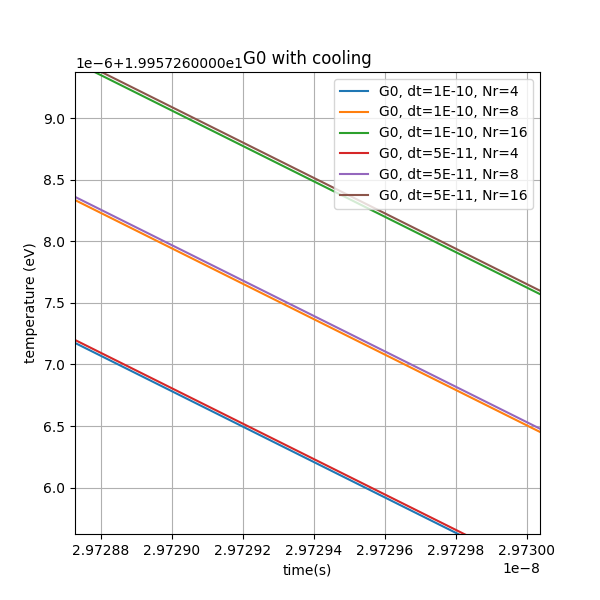
\includegraphics[width=0.99\textwidth]{dat/g0_temp_profile.png}
    \caption{Temperature profile for G0 collision operator with increasing number of polynomials in radial direction with different timestep sizes. The temperature profile curved are grouped based on the number of polynomials used in the radial direction. The above can be expected due to the projection of the infinite dimensional collision operator with finite dimensional approximation. }
\end{figure}

\begin{figure}[H]
    \centering
    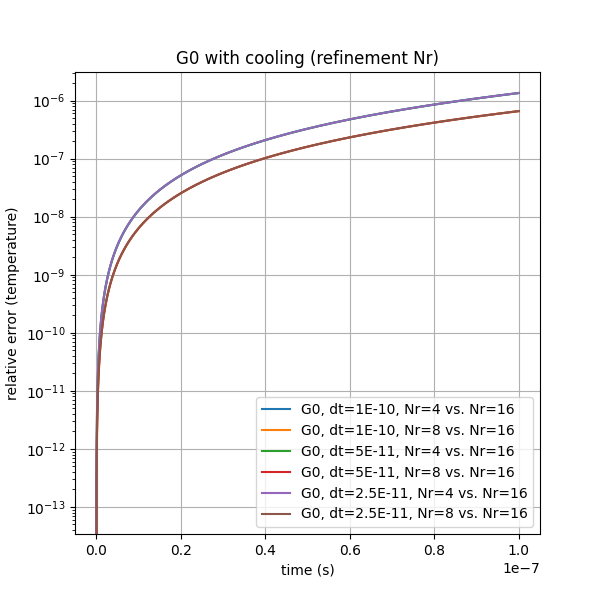
\includegraphics[width=0.99\textwidth]{dat/g0_nr.png}
    \caption{Relative error in the temperature, for G0 collision operator taking $N_r=16$ as the base profile with different timztep sizes of $1E-10$, $5E-11$ and $2.5E-11$. The relative error in the temperature profile, are grouped with respect refinement in the number of radial polynomials used. }
\end{figure}

\begin{table}[H]
    \centering
    \begin{tabular}{|c|c|c|}
        \hline
        $dt$ & $|f_{Nr=4}-f_{Nr=16}|_\infty$ & $|f_{Nr=8}-f_{Nr=16}|_\infty$ \\
        \hline
        1E-10        & 1.35043E-06  &    6.58742E-07 \\
        5E-11        & 1.34977E-06  &    6.58425E-07 \\
        2.5E-11      & 1.35083E-06  &    6.58942E-07 \\
        \hline
    \end{tabular}
    \caption{G0 collision operator : $l_\infty$ norm of the absolute value of the relative error in the temperature profile for a specified timestep size with increasing radial direction approximation order.  }
\end{table}


\begin{figure}[H]
    \centering
    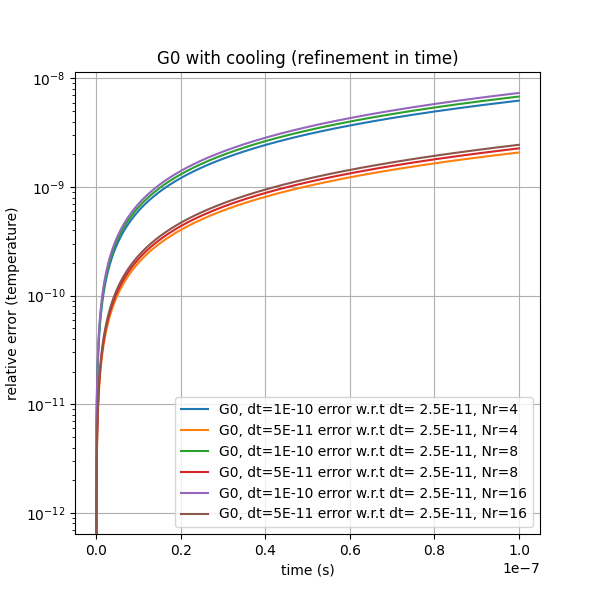
\includegraphics[width=0.99\textwidth]{dat/g0_dt.png}
    \caption{Relative error in the temperature, for G0 collision operator taking $dt=2.5E-11$ as the base profile with different Nr polynomials $Nr=4$, $Nr=8$ and $Nr=16$. The relative error curves are grouped with respect to the refinement in the timestep size. The above shows, for the given finite dimensional approximation of the collision operator, computed temperature profile convergences for a fixed profile.}
\end{figure}

\begin{table}[H]
    \centering
    \begin{tabular}{|c|c|c|}
        \hline
        $Nr$ & $|f_{dt=1E-10}-f_{dt=2.5E-11}|_\infty$ & $|f_{dt=5E-11}-f_{dt=2.5E-11}|_\infty$ \\
        \hline
        4          & 6.24007e-09         & 2.08135e-09 \\
        8          & 6.80473e-09         & 2.26967e-09 \\
        16         & 7.34148e-09         & 2.44868e-09 \\
        \hline
    \end{tabular}
    \caption{G0 collision operator : $l_\infty$ norm of the absolute value of the relative error in the temperature profile for a radial direction approximation order with decreasing timestep size. }
\end{table}

\begin{table}[H]
    \centering
    \begin{tabular}{|c|c|}
        \hline
        $Nr,dt$ & relative error (temperature)\\
        \hline
        Nr=4 dt=1e-10      &           1.35499e-06 \\
        Nr=8 dt=5e-11      &           6.60874e-07 \\
        \hline
    \end{tabular}
    \caption{G0 collision operator : $l_\infty$ norm of the relative error in the temperature profile compared against the $Nr=16$ and $dt=2.5E-11$ case. }
\end{table}

\subsection{G0: $e + Ar \rightarrow e + Ar $  with  G2: $e + Ar \rightarrow e + Ar^+ + e $ (20eV)}
\begin{figure}[H]
    \centering
    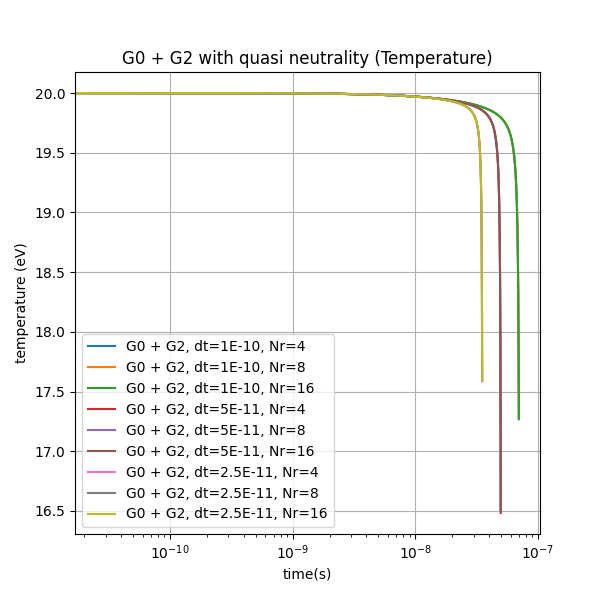
\includegraphics[width=0.99\textwidth]{dat/g02_temp_profile.png}
    \caption{Temperature profile for G0 + G2 collision operator with increasing number of polynomials in radial direction with different timestep sizes. }
\end{figure}

\begin{figure}[H]
    \centering
    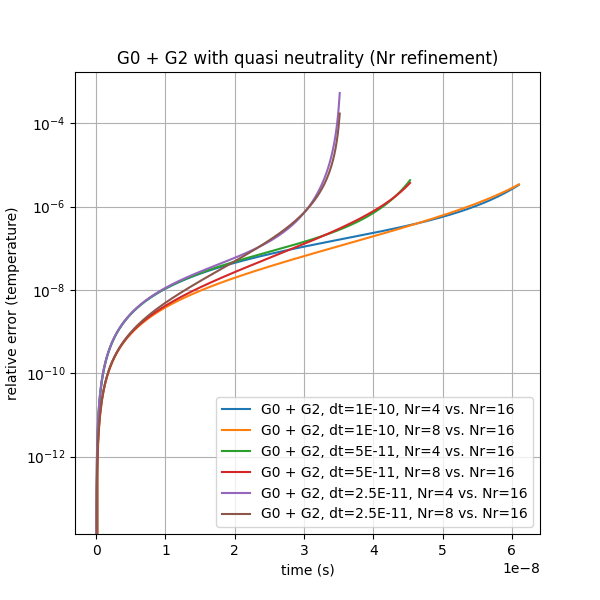
\includegraphics[width=0.99\textwidth]{dat/g02_nr.png}
    \caption{Relative error in the temperature, for G0 + G2 collision operator taking $N_r=16$ as the base profile with different timztep sizes of $1E-10$, $5E-11$ and $2.5E-11$.}
\end{figure}

\begin{table}[H]
    \centering
    \begin{tabular}{|c|c|c|}
        \hline
        $dt$ & $|f_{Nr=4}-f_{Nr=16}|_\infty$ & $|f_{Nr=8}-f_{Nr=16}|_\infty$ \\
        \hline
        1e-10         & 0.0153427        & 0.0024703   \\
        5e-11         & 0.051785         & 0.018351 \\
        2.5e-11       & 0.00773937       & 0.00134626 \\
        \hline
    \end{tabular}
    \caption{G0 + G2 collision operator : $l_\infty$ norm of the absolute value of the relative error in the temperature profile for a specified timestep size with increasing radial direction approximation order. }
\end{table}


\begin{figure}[H]
    \centering
    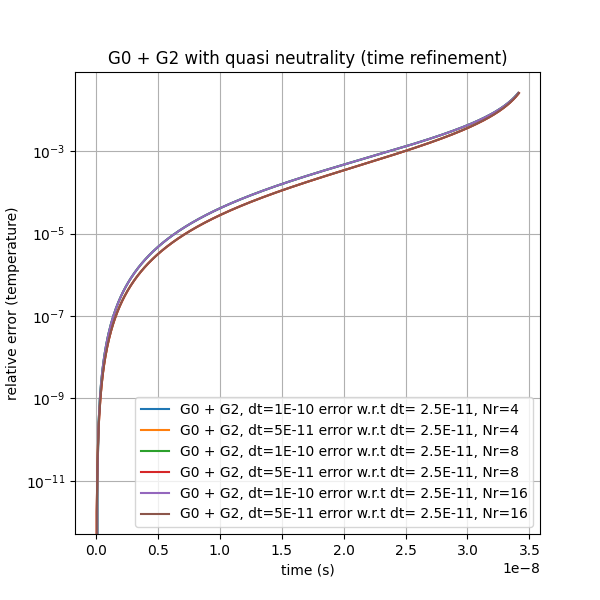
\includegraphics[width=0.99\textwidth]{dat/g02_dt.png}
    \caption{Relative error in the temperature, for G0 + G2 collision operator taking $dt=2.5E-11$ as the base profile with different Nr polynomials $Nr=4$, $Nr=8$ and $Nr=16$.}
\end{figure}

\begin{table}[H]
    \centering
    \begin{tabular}{|c|c|c|}
        \hline
        $Nr$ & $|f_{dt=1E-10}-f_{dt=2.5E-11}|_\infty$ & $|f_{dt=5E-11}-f_{dt=2.5E-11}|_\infty$ \\
        \hline
        4         &   0.0258552           & 0.0257722 \\
        8         &   0.0258221           & 0.0257365 \\
       16        &    0.025834            & 0.0257491 \\
        \hline
    \end{tabular}
    \caption{G0 + G2 collision operator : $l_\infty$ norm of the absolute value of the relative error in the temperature profile for a radial direction approximation order with decreasing timestep size. }
\end{table}

\begin{table}[H]
    \centering
    \begin{tabular}{|c|c|}
        \hline
        $Nr,dt$ & relative error (temperature)\\
        \hline
        Nr=4 dt=1e-10      &           0.25555 \\
        Nr=8 dt=5e-11      &           0.362987 \\
        \hline
    \end{tabular}
    \caption{G0 + G2 (at 20eV) collision operator : $l_\infty$ norm of the relative error in the temperature profile compared against the $Nr=16$ and $dt=2.5E-11$ case. }
\end{table}

\subsection{G0: $e + Ar \rightarrow e + Ar $  with  G2: $e + Ar \rightarrow e + Ar^+ + e $ (1eV)}
\begin{figure}[H]
    \centering
    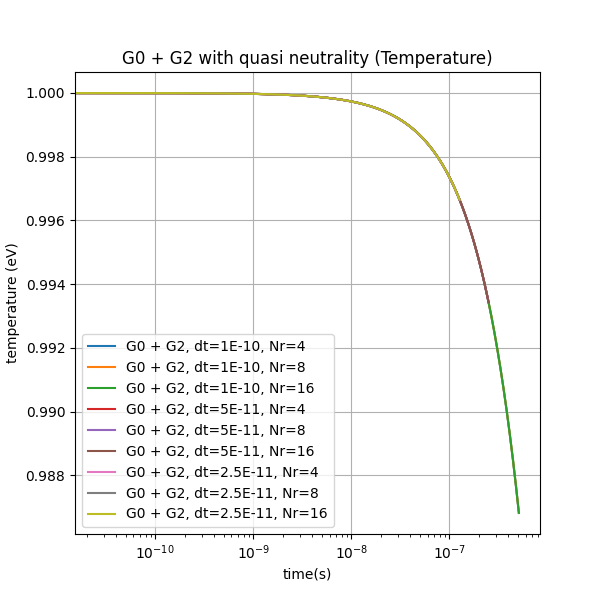
\includegraphics[width=0.49\textwidth]{dat/g012_temp_1ev.png}
    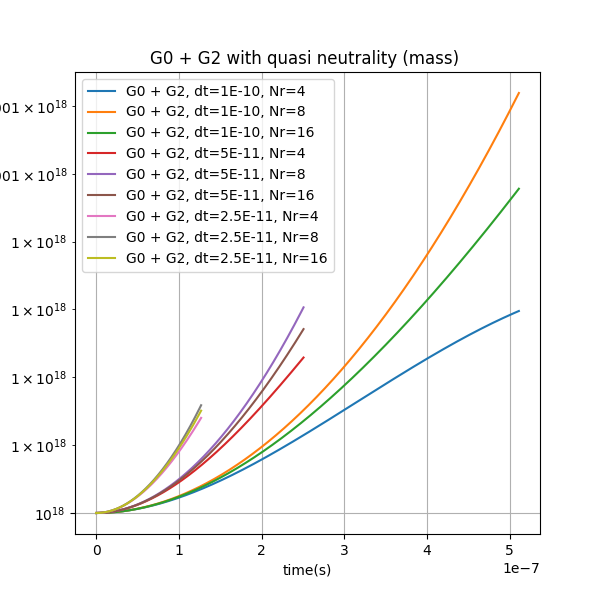
\includegraphics[width=0.49\textwidth]{dat/g012_mass_1ev.png}
    \caption{Temperature (on the left) and the mass (on the right) profiles for G0 + G2 collision operator with increasing number of polynomials in radial direction with different timestep sizes. }
\end{figure}

\begin{figure}[H]
    \centering
    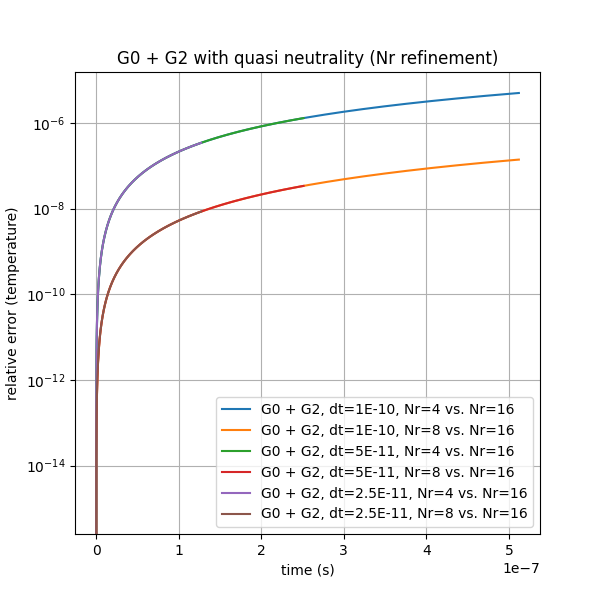
\includegraphics[width=0.99\textwidth]{dat/g02_nr_1ev.png}
    \caption{Relative error in the temperature, for G0 + G2 collision operator taking $N_r=16$ as the base profile with different timztep sizes of $1E-10$, $5E-11$ and $2.5E-11$.}
\end{figure}

\begin{figure}[H]
    \centering
    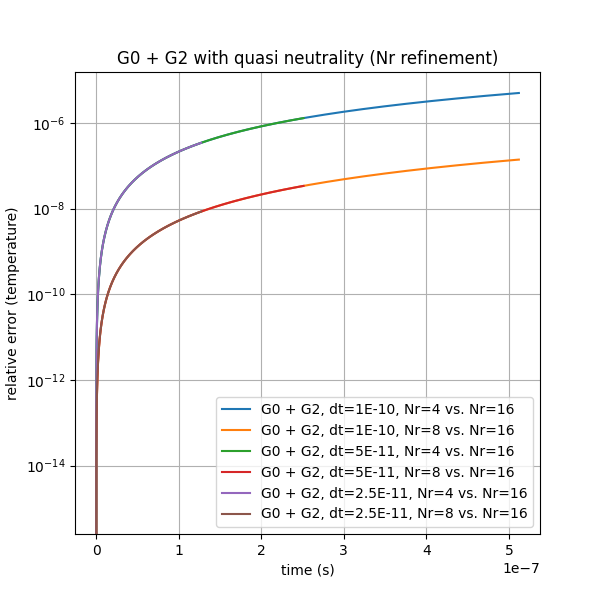
\includegraphics[width=0.99\textwidth]{dat/g02_nr_1ev.png}
    \caption{Relative error in the temperature, for G0 + G2 collision operator taking $dt=2.5E-11$ as the base profile with different Nr polynomials $Nr=4$, $Nr=8$ and $Nr=16$.}
\end{figure}


\begin{table}[H]
    \centering
    \begin{tabular}{|c|c|}
        \hline
        $Nr,dt$ & relative error (temperature)\\
        \hline
        Nr=4 dt=1e-10         &       3.56035e-07 \\
        Nr=8 dt=5e-11         &       1.3401e-08   \\
        \hline
    \end{tabular}
    \caption{G0 + G2 (at 1eV) collision operator : $l_\infty$ norm of the relative error in the temperature profile compared against the $Nr=16$ and $dt=2.5E-11$ case. }
\end{table}



\bibliographystyle{plain}
\bibliography{bte_notes.bib}

\appendix

\section{Derivation of Collision operators}

\subsection{Binary reactions}

We start with reactions of the type
\begin{align*}
\text{Ar} + e \longrightarrow \tilde{\text{Ar}} + e
\end{align*}
where $\tilde{\text{Ar}} = \text{Ar}$ in the case of elastic collisions and $\tilde{\text{Ar}} = \text{Ar}^\ast$ in the case of excitation events. Let us denote the expressions that map given pre-collisional velocities $\vect{v}_e$, $\vect{v}_0$ to post-collisional velocities as 
\begin{align*}
\vect{v}_e^\text{post} &= \vect{v}_e^\text{post} \of{\vect{v}_e, \vect{v}_0, \vect{\omega}}
\\
\vect{v}_0^\text{post} &= \vect{v}_0^\text{post} \of{\vect{v}_e, \vect{v}_0, \vect{\omega}}
\end{align*} 
where $\vect{\omega} \in S^2$ is the vector defining along which directions velocities change in the reaction. Specifically, from the conservation of momentum and energy it can be derived that
\begin{align*}
\vect{v}_e^\text{post} &= \vect{v}_e + \frac{\alpha}{m_e}\vect{\omega},
\\
\vect{v}_0^\text{post} &= \vect{v}_0 - \frac{\alpha}{m_0}\vect{\omega},
\end{align*}
where
\begin{align*}
\alpha &= \frac{u + \sqrt{u^2 - 4 \Delta E \mu}}{2\mu},
\quad 
u = \vect{\omega} \cdot \left( \vect{v}_0 - \vect{v}_e \right),
\quad 
\mu = \frac{m_e+m_0}{2 m_e m_0}
\end{align*}
and $\Delta E$ denotes the energy loss during the reaction ($\Delta E = 0$ for elastic collisions). The inverse map (assuming it exists and well-defined) is denoted as 
\begin{align*}
\vect{v}_e^\text{pre} &= \vect{v}_e^\text{pre} \of{\vect{v}_e, \vect{v}_0, \vect{\omega}}
\\
\vect{v}_0^\text{pre} &= \vect{v}_0^\text{pre} \of{\vect{v}_e, \vect{v}_0, \vect{\omega}}
\end{align*} 
where $\vect{v}_e$, $\vect{v}_0$ now represent the post-collision velocities. Thus we have 
\begin{align*}
\vect{v}_e &= \vect{v}_e^\text{pre} \of{\vect{v}_e^\text{post} \of{\vect{v}_e, \vect{v}_0, \vect{\omega}}, \vect{v}_0^\text{post} \of{\vect{v}_e, \vect{v}_0, \vect{\omega}}, \vect{\omega}}
\\
\vect{v}_0 &= \vect{v}_0^\text{pre} \of{\vect{v}_e^\text{post} \of{\vect{v}_e, \vect{v}_0, \vect{\omega}}, \vect{v}_0^\text{post} \of{\vect{v}_e, \vect{v}_0, \vect{\omega}}, \vect{\omega}}
\end{align*} 

Let us denote the collision kernel of reaction as $B\of{\vect{v}_e, \vect{v}_0, \vect{\omega}}$ which is a function of pre-collision velocities $\vect{v}_e$, $\vect{v}_0$ and the direction of velocity change $\vect{\omega}$. The number of electrons with velocity $\vect{v}_e$ that will participate in the reaction and, thus, lost is given by 
\begin{align*}
C^- = \int_{R^3} \int_{S^2} B\of{\vect{v}_e, \vect{v}_0, \vect{\omega}} f_e\of{\vect{v}_e} f_0\of{\vect{v}_0} \diff{\vect{v}_0} \diff{\vect{\omega}}
\end{align*}
The number of electrons with the same velocity created in the reaction is given by
\begin{align*}
C^+ = \int_{R^3} \int_{R^3} \int_{S^2} 
B\of{\vect{v}_e^\prime, \vect{v}_0^\prime, \vect{\omega}} 
f_e\of{\vect{v}_e^\prime} f_0\of{\vect{v}_0^\prime} 
\delta\of{\vect{v}_e^\text{post}\of{\vect{v}_e^\prime, \vect{v}_0^\prime, \vect{\omega}} - \vect{v}_e} 
\diff{\vect{v}_0^\prime} \diff{\vect{v}_e^\prime} \diff{\vect{\omega}}
\end{align*}
where we integrate over all possible pre-collision velocities $\vect{v}_e^\prime$, $\vect{v}_0^\prime$ but pick out only those that result in post-collision electron velocity $\vect{v}_e$ (thanks to the delta function). Note that in the expression for $C^-$ symbols $\vect{v}_e$, $\vect{v}_0$ have the meaning of pre-collision velocity, while in the expression for $C^+$ those are denoted by $\vect{v}_e^\prime$, $\vect{v}_0^\prime$. 

\textbf{Remark.} One could define $C^-$ in an analogous to $C^+$ way. That is, consider reactions for all possible pre-collision velocities $\vect{v}_e^\prime$, $\vect{v}_0^\prime$ but select only those that lead to loss of electrons with velocity $\vect{v}_e$
\begin{align*}
C^- = \int_{R^3} \int_{R^3} \int_{S^2} 
B\of{\vect{v}_e^\prime, \vect{v}_0^\prime, \vect{\omega}} 
f_e\of{\vect{v}_e^\prime} f_0\of{\vect{v}_0^\prime} 
\delta\of{\vect{v}_e^\prime - \vect{v}_e} 
\diff{\vect{v}_0^\prime} \diff{\vect{v}_e^\prime} \diff{\vect{\omega}}.
\end{align*}

We understand $C^-$ and $C^+$ as operators acting on functions of variable $\vect{v}_e$. Their weak forms are given by
\begin{align*}
\int_{R^3} C^- \phi\of{\vect{v}_e} \diff{\vect{v}_e} 
&=
\int_{R^3} \int_{R^3} \int_{S^2} 
B\of{\vect{v}_e, \vect{v}_0, \vect{\omega}} 
f_e\of{\vect{v}_e} f_0\of{\vect{v}_0} 
\phi\of{\vect{v}_e} 
\diff{\vect{v}_e} \diff{\vect{v}_0} \diff{\vect{\omega}}
\\
\int_{R^3} C^+ \phi\of{\vect{v}_e} \diff{\vect{v}_e} 
&= 
\int_{R^3} \int_{R^3} \int_{S^2} 
B\of{\vect{v}_e^\prime, \vect{v}_0^\prime, \vect{\omega}} 
f_e\of{\vect{v}_e^\prime} f_0\of{\vect{v}_0^\prime} 
\phi\of{\vect{v}_e^\text{post}\of{\vect{v}_e^\prime, \vect{v}_0^\prime, \vect{\omega}}} 
\diff{\vect{v}_0^\prime} \diff{\vect{v}_e^\prime} \diff{\vect{\omega}}
\\
&= 
\int_{R^3} \int_{R^3} \int_{S^2} 
B\of{\vect{v}_e, \vect{v}_0, \vect{\omega}} 
f_e\of{\vect{v}_e} f_0\of{\vect{v}_0} 
\phi\of{\vect{v}_e^\text{post}\of{\vect{v}_e, \vect{v}_0, \vect{\omega}}} 
\diff{\vect{v}_0} \diff{\vect{v}_e} \diff{\vect{\omega}}
\end{align*}
where we integrated out the delta function and renamed dummy variables. Thus the weak form of the total collision operator $C = C^+ - C^-$ can be written as 
\begin{align*}
\int_{R^3} C \phi\of{\vect{v}_e} \diff{\vect{v}_e} 
&=
\int_{R^3} \int_{R^3} \int_{S^2} 
B\of{\vect{v}_e, \vect{v}_0, \vect{\omega}} 
f_e\of{\vect{v}_e} f_0\of{\vect{v}_0} 
\left(
\phi\of{\vect{v}_e^\text{post}\of{\vect{v}_e, \vect{v}_0, \vect{\omega}}} 
- \phi\of{\vect{v}_e} 
\right)
\diff{\vect{v}_0} \diff{\vect{v}_e} \diff{\vect{\omega}}
\end{align*}

While for our purposes this formulation is all we need, for completeness sake we derive a strong form of the collision operator. To do so, we perform a change of variables in the weak form of gain operator $C^+$ according to:
\begin{align*}
\vect{v}_e^\prime &= \vect{v}_e^\text{pre} \of{\vect{v}_e^{\prime\prime}, \vect{v}_0^{\prime\prime}, \vect{\omega}}
\\
\vect{v}_0^\prime &= \vect{v}_0^\text{pre} \of{\vect{v}_e^{\prime\prime}, \vect{v}_0^{\prime\prime}, \vect{\omega}}
\end{align*}
As result we get
\begin{multline*}
\int_{R^3} C^+ \phi\of{\vect{v}_e} \diff{\vect{v}_e} 
= 
\int_{R^3} \int_{R^3} \int_{S^2} 
B\of{\vect{v}_e^\text{pre} \of{\vect{v}_e^{\prime\prime}, \vect{v}_0^{\prime\prime}, \vect{\omega}}, \vect{v}_0^\text{pre} \of{\vect{v}_e^{\prime\prime}, \vect{v}_0^{\prime\prime}, \vect{\omega}}, \vect{\omega}} 
\times
\\
\times
f_e\of{\vect{v}_e^\text{pre} \of{\vect{v}_e^{\prime\prime}, \vect{v}_0^{\prime\prime}, \vect{\omega}}} 
f_0\of{\vect{v}_0^\text{pre} \of{\vect{v}_e^{\prime\prime}, \vect{v}_0^{\prime\prime}, \vect{\omega}}} 
\phi\of{\vect{v}_e^{\prime\prime}} 
|J\of{\vect{v}_e^{\prime\prime}, \vect{v}_0^{\prime\prime}, \vect{\omega}}|
\diff{\vect{v}_0^{\prime\prime}} \diff{\vect{v}_e^{\prime\prime}} \diff{\vect{\omega}}
\end{multline*}
or, after renaming dummy variables,
\begin{multline*}
\int_{R^3} C^+ \phi\of{\vect{v}_e} \diff{\vect{v}_e} 
= 
\int_{R^3} \int_{R^3} \int_{S^2} 
B\of{\vect{v}_e^\text{pre} \of{\vect{v}_e, \vect{v}_0, \vect{\omega}}, \vect{v}_0^\text{pre} \of{\vect{v}_e, \vect{v}_0, \vect{\omega}}, \vect{\omega}} 
\times
\\
\times
f_e\of{\vect{v}_e^\text{pre} \of{\vect{v}_e, \vect{v}_0, \vect{\omega}}} 
f_0\of{\vect{v}_0^\text{pre} \of{\vect{v}_e, \vect{v}_0, \vect{\omega}}} 
\phi\of{\vect{v}_e} 
|J\of{\vect{v}_e, \vect{v}_0, \vect{\omega}}|
\diff{\vect{v}_0} \diff{\vect{v}_e} \diff{\vect{\omega}}
\end{multline*}
where $J\of{\vect{v}_e, \vect{v}_0, \vect{\omega}} = \frac{ \partial \left( \vect{v}_e^\text{pre}\of{\vect{v}_e, \vect{v}_0, \vect{\omega}}, \vect{v}_0^\text{pre}\of{\vect{v}_e, \vect{v}_0, \vect{\omega}} \right)}{\partial \left( \vect{v}_e, \vect{v}_0 \right)}$ is the Jacobian of the transformation of variables. Note that in this last expression $\vect{v}_e$, $\vect{v}_0$ can be interpreted as post-collision velocities. Combining it with the weak form of the loss operator (where $\vect{v}_e$, $\vect{v}_0$ actually stand for pre-collision velocities) we obtain
\begin{multline*}
\int_{R^3} C \phi\of{\vect{v}_e} \diff{\vect{v}_e} 
=
\int_{R^3} \int_{R^3} \int_{S^2} 
\phi\of{\vect{v}_e} 
\diff{\vect{v}_0} \diff{\vect{v}_e} \diff{\vect{\omega}}
\times
\\
\times
\big(
B^\text{pre}\of{\vect{v}_e, \vect{v}_0, \vect{\omega}}  
f_e^\text{pre}\of{\vect{v}_e, \vect{v}_0, \vect{\omega}}
f_0^\text{pre}\of{\vect{v}_e, \vect{v}_0, \vect{\omega}} 
|J\of{\vect{v}_e, \vect{v}_0, \vect{\omega}}|
\\
-
B\of{\vect{v}_e, \vect{v}_0, \vect{\omega}} 
f_e\of{\vect{v}_e} f_0\of{\vect{v}_0} 
\big)
\end{multline*}
where notation $x^\text{pre}\of{\vect{v}_e, \vect{v}_0, \vect{\omega}} = x\of{\vect{v}_e^\text{pre} \of{\vect{v}_e, \vect{v}_0, \vect{\omega}}, \vect{v}_0^\text{pre} \of{\vect{v}_e, \vect{v}_0, \vect{\omega}}, \vect{\omega}}$ is used. Thus, a strong form of the total collision operator for general binary reactions can be written as
\begin{align*}
C = 
\int_{R^3} \int_{S^2} 
\left(
f_e^\text{pre}
f_0^\text{pre}
B^\text{pre} 
|J|
-
f_e
f_0
B
\right)
\diff{\vect{v}_0} \diff{\vect{\omega}}
\end{align*}
In case of elastic collisions it can be shown that $|J| = 1$ and
\begin{align*}
B^\text{pre}\of{\vect{v}_e, \vect{v}_0, \vect{\omega}} &=
B\of{\vect{v}_e^\text{pre} \of{\vect{v}_e, \vect{v}_0, \vect{\omega}}, \vect{v}_0^\text{pre} \of{\vect{v}_e, \vect{v}_0, \vect{\omega}}, \vect{\omega}} 
\\
&=
B\of{|\vect{v}_e^\text{pre}- \vect{v}_0^\text{pre}|, |\left(\vect{v}_e^\text{pre}- \vect{v}_0^\text{pre}\right)\cdot\vect{\omega}|} 
\\
&=
B\of{|\vect{v}_e- \vect{v}_0|, |\left(\vect{v}_e- \vect{v}_0\right)\cdot\vect{\omega}|}
\\
&=
B\of{\vect{v}_e, \vect{v}_0, \vect{\omega}} 
\end{align*}
and the collision operator becomes the familiar
\begin{align*}
C = 
\int_{R^3} \int_{S^2} 
\left(
f_e^\text{pre}
f_0^\text{pre}
-
f_e
f_0
\right)
B
\diff{\vect{v}_0} \diff{\vect{\omega}}
\end{align*}
\end{document}
